\chapter{Esercizio 8}

\subsection{Testo}

\begin{center}
    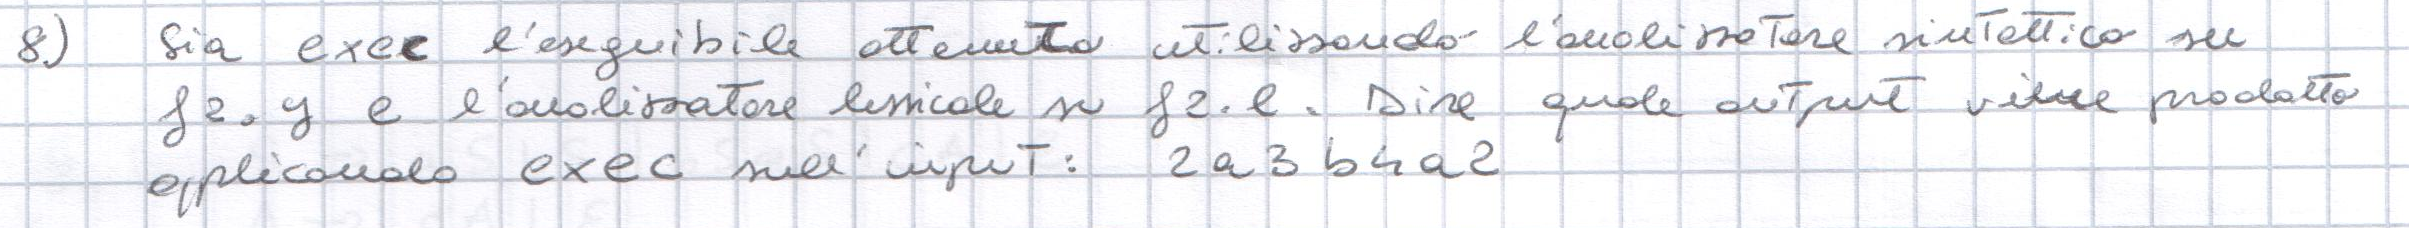
\includegraphics[scale=0.2]{Chapters/Img/08text.png}\\
\end{center} 

\subsection{Soluzione}
f2.y
\begin{lstlisting}
    %{
    #include <stdio.h>
    #include <stdlib.h>
    
    int yylex();
    int yyparse();
    void yyerror(char *s);

    %}

    %token a b num

    %%
    S: S E '\n' { printf("%d\n", $2); }
    | ;
    E: num { $$ = $1; }
    | E a E { $$ = $1 * $3; }
    | E b E { $$ = $1 + $3; } ;
    %%

    int main() {
    yyparse();
    return 0;
    }

    void yyerror(char *s) {
    printf("Error when reading: %s", s);
    }
\end{lstlisting}

f2.l
\begin{lstlisting}
    %option noyywrap

    %{
    #include "y.tab.h"
    #include <stdio.h>
    %}

    %%

    "a"   { return a; }
    "b"   { return b; }
    [0-9]+  { yylval = atoi(yytext); return num; }
    [-+\n]  return *yytext;
    [ \t]  ;
    .   yyerror("Invalid character");

    %%
\end{lstlisting}

\subsection{Risposta}
Input: 2a3b4a2
Output: 22